\subfigure[Sprout Segments]{
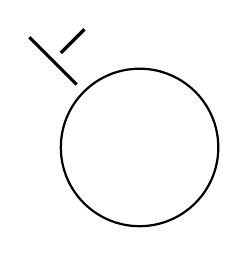
\begin{tikzpicture}
	\node [draw, thick, circle, text centered,  minimum size=2cm] at (0,0) {}; 
	%% BL Sprout
	\draw [very thick] (-0.8,0.8) -- +(-0.6,0.6);
	\draw [very thick] (-1,1.2) -- +(0.3,0.3);
	%\node at (-1.2, -2) {$(d)$};
\end{tikzpicture}
}
\subfigure[Branching]{
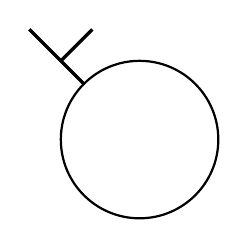
\begin{tikzpicture}
	\node [draw, thick, circle, text centered,  minimum size=2cm] at (0,0) {}; 
	%% TL Sprout
	\draw [very thick] (-0.7,0.7) -- +(-0.7,0.7);
	\draw [very thick] (-1,1) -- +(0.4,0.4);
	%\node at (-1, 2) {$(c)$};
\end{tikzpicture}
}
\subfigure[Junction Point]{
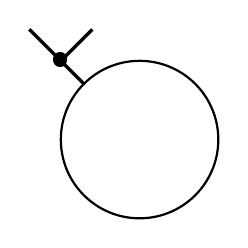
\begin{tikzpicture}
	\node [draw, thick, circle, text centered,  minimum size=2cm] at (0,0) {}; 
	%% TL Sprout
	\draw [very thick] (-0.7,0.7) -- +(-0.7,0.7);
	\draw [very thick] (-1,1) -- +(0.4,0.4);
	\node at (-1,1) {\Large\textbullet};
	%\node at (-1, 2) {$(c)$};
\end{tikzpicture}
}
